The interaction of particles with matter is described in this section, focusing on the particles and energy range relevant for this thesis, electrons ($0-18~\keV$), photons in the visible range (approx. $380-750~\nm$) and $\gamma$ rays from the background and high energy cosmic rays.

Electrons have a charge, so their interaction with matter is mainly through the orbital atomic  electrons by the Coulomb force. The electron trajectories are much more tortuous than those of heavier particles because of their small mass. Furthermore, electrons lose a significant amount of energy in each collision. The specific energy loss, defined as $S=-\displaystyle{\frac{dE}{dx}}$, gives the energy loss of a particle per unit of path length. In the case of electrons, the total energy loss has two main contributions, the collisions (elastic and inelastic) and the radiative processes (bremsstrahlung) which are roughly proportional \cite{Knoll, Leo},
\begin{equation}
\frac{dE}{dx} \approx \left(\frac{dE}{dx}\right)_{c} + \left(\frac{dE}{dx}\right)_{br} ; \qquad \frac{\displaystyle{\left(\frac{dE}{dx}\right)_{br}}}{\displaystyle{\left(\frac{dE}{dx}\right)_{c}}} \approx \frac{EZ}{700}
\label{eq:ElectronInteraction}
\end{equation}
where $E$ is the energy of the electron in $\MeV$ and $Z$ is the atomic number of the absorbing material. Due to this energy loss, electrons penetrate a material to a depth where they have lost their kinetic energy. This distance, known as the range, is quoted for tritium electrons in Table \ref{tab:MeanFreePathTritium}. 

The material chosen for the detection of tritium decay electrons is organic plastic since, due to its low density, there is a reduced backscattering. It has been chosen in the form of fibres in order to increase the active area and, therefore, the efficiency of the detector.

As photons do not have any charge, their possible interactions with matter are the photoelectric effect, Compton effect, coherent scattering and pair production. The probability of each process, displayed in Figure \ref{fig:ProcessesPhotons}, depends on the energy of the photon, $E_\gamma = h\nu$, and on the atomic number of the material, Z. The optical photons have a wavelength between $400$ and $700~\nano\meter$, that corresponds to energies of the order of the $\eV$. Therefore, pair production does not play any role for optical photons since this requires photon energy of at least $1.022~\MeV$.

\begin{figure}[h]
\centering
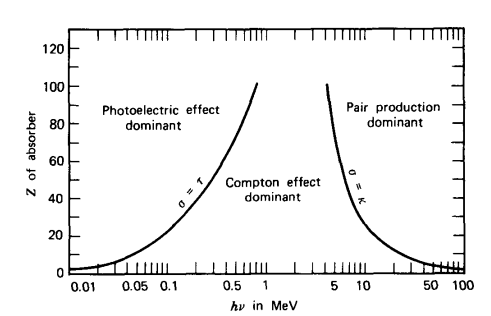
\includegraphics[scale=0.75]{3DesignPrinciples/32Tritium_detector/DominantProcessesPhotons.png}
\caption{Domain regions of the three most probable types of interactions of gamma rays with matter. The lines show the atomic number $Z$ and gamma energy $h\nu$ where two interaction processes are equally likely\label{fig:ProcessesPhotons}~\cite{Knoll}.}
\end{figure}

The photoelectric effect occurs when a photon interacts with an orbital electron in the material, losing all its energy. This energy is absorbed by an electron that is ejected from the atom (ionization). The energy of the resulting electron, $E_e$, is \cite{Knoll, Leo},
\begin{equation}
E_e = E_\gamma - E_b 
\label{eq:PhotoelectricEffect}
\end{equation}
where $E_b$ is the binding energy of the electron in the material. The probability of this effect depends on the number of available electrons in matter through the atomic number $Z$, and the energy of the electron according to the expression \cite{Knoll},
\begin{equation}
\tau \approx \frac{Z^n}{E_\gamma^{3.5}}
\label{eq:PhotoelectricProb}
\end{equation}
Thus, the photoelectric effect is most probable for elements with a high atomic number. This is the reason why these types of elements are the best shields against gamma radiation and why the passive shield of the TRITIUM monitor consists of lead bricks (section \ref{subsec:SetUpPassiveShield}). %This is also the reason why elements with high atomic number like $\ce{Sb}$ ($Z=51$), $\ce{Rb}$ ($Z=37$) or $\ce{Cs}$ ($Z=55$), are used in the cathodes of PMTs. 

The Compton effect occurs when a photon interacts with an orbital electron of the material, transferring part of its energy to the electron which is scattered at an angle $\theta$ with respect to the direction of the incident photon. If the electron binding energy is neglected, the energy transferred to it, $E_e$, is given by \cite{Knoll, Leo},
\begin{equation}
E_e=\frac{\displaystyle{\frac{E_\gamma^2}{m_0c^2}}\left(1-cos\theta\right)}{1+ \displaystyle{\frac{E_\gamma^2}{m_0c^2}}\left(1-cos\theta\right)}
\label{eq:ComptonEffect}
\end{equation}
where $m_0$ is the rest mass of the electron and $c$ is the speed of light in the vacuum. The probability of the Compton effect is proportional to the atomic number $Z$  and decreases with the energy of the photon. As it can be seen in Figure \ref{fig:ProcessesPhotons}, for photon energies in the visible spectrum (of the order of eV), the Compton effect is only likely for very light materials ($Z<4$). For heavier materials the photoelectric effect is dominant.

In the coherent scattering, the atom is neither excited nor ionized and the photon conserves its energy in the collision. Coherent scattering is probable for photons with low energies and materials with high atomic numbers. % and, as it will be shown in section \ref{subsec:PlasticScintillators}, it explains why the produced photons are guided along scintillating fibres. 

Finally, in the pair production process, the photon is converted into an electron and a positron,
\begin{equation}
\gamma \longrightarrow e^- ~ + ~ e^+
\label{eq:pairproductionprocess}
\end{equation}
As can be seen in Figure \ref{fig:ProcessesPhotons}, this is the dominant interaction process for high-energy photons, which are the photons produced by cosmic rays.


%Because of the fact that the energy of the photon doesn't change we will not speak more about this effect but it is important since this effect change de direction of photons and it will affect to their mean free path.